\section{Mapa conceptual}

El siguiente mapa conceptual relaciona los ocho conceptos centrales de esta investigación, siguiendo las mismas decisiones de diseño explicadas en el resto del informe.

\begin{figure}[H]
    \centering
    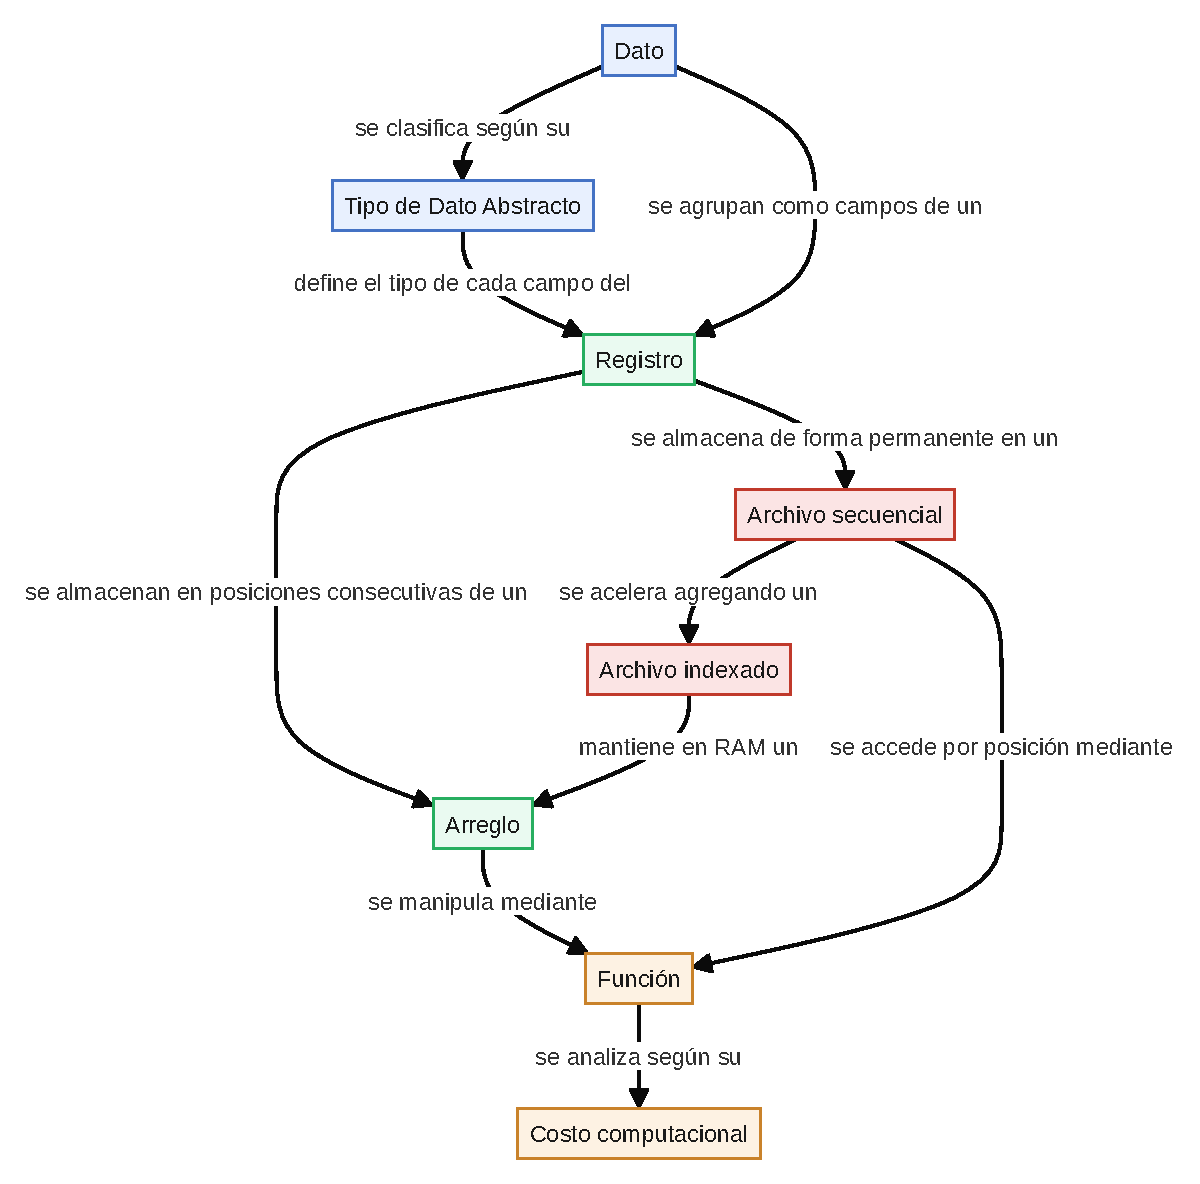
\includegraphics[width=\textwidth]{../diagramas/output/mapa-conceptual.pdf}
    \caption{Mapa conceptual de la investigación}
    \label{fig:mapa-conceptual}
\end{figure}

Un \textbf{Dato} sin clasificar no dice mucho por sí solo: primero se clasifica según su \textbf{Tipo de Dato Abstracto} (entero, cadena, fecha, enumerado), y ese tipo es lo que define cómo se declara cada campo del \textbf{Registro}. Varios registros consecutivos forman un \textbf{Arreglo}, que en este sistema vive tanto en disco (los tres archivos de tamaño fijo) como en RAM (el mapa de posiciones).

Sobre ese arreglo operan las \textbf{Funciones} documentadas en las secciones anteriores, y cada una de ellas se analiza según su \textbf{Costo computacional} en notación Big O, tal como exige el caso de estudio.

Los registros no viven solo en memoria: se guardan de forma permanente en un \textbf{Archivo secuencial}, accesible por posición mediante funciones como \texttt{fseek} y \texttt{fread}. Para no tener que recorrerlo completo en cada búsqueda, ese archivo se acelera agregando un \textbf{Archivo indexado}, que a su vez es justamente el que mantiene en RAM el arreglo (mapa de posiciones) mencionado antes, cerrando el ciclo entre los ocho conceptos.
